\documentclass[a4paper,12pt]{article} % добавить leqno в [] для нумерации слева
\usepackage[a4paper,top=1.3cm,bottom=2cm,left=1.5cm,right=1.5cm,marginparwidth=0.75cm]{geometry}
%%% Работа с русским языком
\usepackage{cmap}					% поиск в PDF
\usepackage{mathtext} 				% русские буквы в фомулах
\usepackage[T2A]{fontenc}			% кодировка
\usepackage[utf8]{inputenc}			% кодировка исходного текста
\usepackage[english,russian]{babel}	% локализация и переносы

\usepackage{graphicx}
\usepackage{mathtools}
\usepackage{wrapfig}
\usepackage{tabularx}
\usepackage{amssymb}
\usepackage{hyperref}
\usepackage[rgb]{xcolor}
\hypersetup{colorlinks=true,urlcolor=blue}
%% Шрифты
\usepackage{euscript}	 % Шрифт Евклид
\usepackage{amsmath}
\usepackage{mathtools}
%%% Заголовок
\author{Lokhmatov Arseniy}
\title{Лабораторная работа по общей физике}

\date{\today}
\begin{document}
\begin{titlepage}
    \newpage
    \begin{center}
    {\large МОСКОВСКИЙ ФИЗИКО-ТЕХНИЧЕСКИЙ ИНСТИТУТ (НАЦИОНАЛЬНЫЙ ИССЛЕДОВАТЕЛЬСКИЙ УНИВЕРСИТЕТ)}
    \vspace{1cm}

    {\largeФизтех-школа аэрокосмических технологий}
    \vspace{6em}
    \end{center}
    
    \vspace{1.2em}

    \begin{center}
    %\textsc{\textbf{}}
    \Large Лабораторная работа №3.4.1 \\
    Измерение магнитной восприимчивости диа- и парамагнетиков 
    \linebreak
    \end{center}
    
    \vspace{11em}
    
    \begin{flushright}
                       {\large Работу выполнил\\
                       Лохматов Арсений Игоревич\\
                       Козярский Алексей Сергеевич\\
                       Б03-303 }
    \end{flushright}

    \vspace{\fill}

    \begin{center}
        
\includegraphics[width=0.2\linewidth]{dasr.png}
    \end{center}

    \begin{center}
    Долгопрудный, 2024
    \end{center}

    \end{titlepage}

\section{Теоретическая часть}

\paragraph{Цель работы:} измерить магнитную восприимчивость диа- и парамагнетиков.

\paragraph{Оборудование:} электромагнит, весы, милливеберметр, регулируемый источник постоянного тока, образцы диа- и парамагнетиков.

\subsection{Экспериментальная установка}

Схема установки приведена на рисунке \ref{img1}. Магнитное поле с максимальной индукцией $\simeq 1 \text{ Т}$ создаётся в зазоре электромагнита, питаемого постоянным током. Диаметр полюсов существенно превосходит ширину зазора, поэтому поле в средней части зазора достаточно однородно. Величина тока, проходящего через обмотки электромагнита, задаётся регулируемым источником питания и измеряется амперметром, встроенным в источник питания. Градуировка электромагнита производится при помощи милливеберметра.

\begin{figure}[h]
\begin{center}
		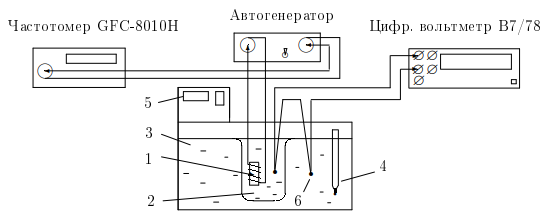
\includegraphics[width=8cm]{card1.png}
\end{center}
	\caption{Схема установки}
	\label{img1}
\end{figure}

При измерениях образцы поочердно подвешиваются к весам так, что один конеч образца оказывается в зазоре электромагнита, а другой - вне зазора, где индукцией магнитного поля можно пренебречь. При помощи весов определяется перегрузка $\Delta P = F$ -- сила, действующая на образец со стороны магнитного поля.

Силы, действующие на диа- парамагнитные образцы, очень малы.

\newpage

\section{Практическая часть}

В работе предлагается исследовать зависимость силы, действующей на образец, размещённый в зазор элетромагнита, от величины поля в зазоре и по результатам измерений рассчитать магнитную восприимчивость меди и аллюминия.

\subsection{Подготовка приборов к работе}

\begin{enumerate}
    \item Включим в сеть весы для прогрева.
    \item Ознакомимся с экспериментальной установкой, изображённой на рисунке \ref{img1}, и техническим описанием источника питания.
    \item Проверим работу цепи питания магнита: для этого пере включением источника питания убедимся в том, что
    \begin{enumerate}
        \item все регулировочные ручки источника питания установлены на минимум;
        \item включим источник питания в сеть и установим обе ручки регулировки \textbf{напряжения} на максимум;
        \item для увеличения тока через магнит сначала выведем ручку плавной регулировки \textbf{тока "fine"} до максимума, потом ручку грубой регулировки \textbf{"coarse"}, уменьшение тока производится в обратном порядке. 
    \end{enumerate}
    Определим максимально возможный ток через магнит $I_{max}$ и уберм ток до нуля.

    \[ I_{max} = (1.17 \pm 0.02) \text{ А } (\varepsilon = 1.7\%) \]
    
\end{enumerate}

\subsection{Калибровка магнита $[B = f(I)]$}

\begin{enumerate}
    \item Ознакомились с описанием милливеберметра.
    \item Определим зависимость индукции $B$ в зазоре от тока, протекающего через обмотку электромагнита. Для этого устанавливаем силу тока в электромагните, вносим пробную катушку милливеберметра в магнитное поле катушки, устаноавливаем начальное значение милливеберметра, быстро вынимаем датчик и записываем разность показаний милливеберметра до и после вынимания катушки. Чтобы данное значение перевести в величину магнитной индукции, пользуемся соотношением:

\[ dW = B\cdot SN \Longleftrightarrow B = \frac{dW}{SN}, \text{ } SN = 72 \text{ см}^2. \]

Результаты измерений занесём в таблицу \ref{tab1}.

\begin{table}[h]
	\centering
	\begin{tabular}{|c|c|c|}
		\hline
		$ I, \text{ А}$ & $ W, \text{ мВб}$ & $B, \text{ Тл}$ \\ \hline
		0.2 & 1.5 & 0.208 \\ \hline
            0.3 & 2.2 & 0.306 \\ \hline
            0.4 & 2.9 & 0.403 \\ \hline
            0.5 & 3.6 & 0.5 \\ \hline
            0.6 & 4.4 & 0.611 \\ \hline
	\end{tabular}
        \begin{tabular}{|c|c|c|}
		\hline
		$ I, \text{ А}$ & $ W, \text{ мВб}$ & $B, \text{ Тл}$ \\ \hline
		0.7 & 5.05 & 0.701 \\ \hline
            0.8 & 5.65 & 0.785 \\ \hline
            0.9 & 6.3 & 0.875 \\ \hline
            1.0 & 6.85 & 0.951 \\ \hline
            1.1 & 7.3 & 1.014 \\ \hline
	\end{tabular}
        
	\caption{Градуировка электромагнита}
	\label{tab1}
\end{table}

По полученным данным построим график зависимости $ B=f(I) $. 

\begin{figure}[h]
    \begin{center}
		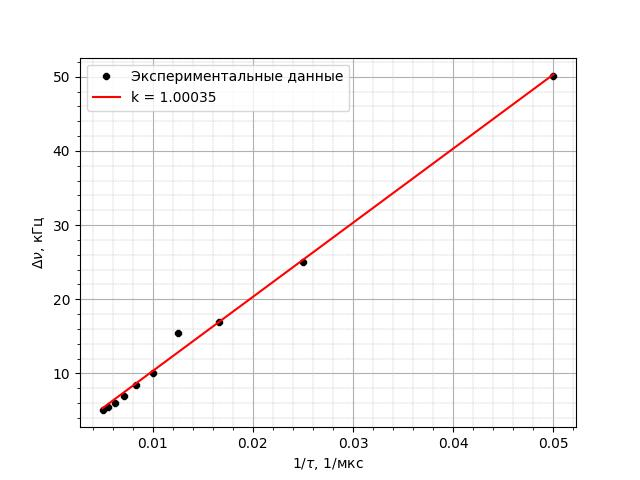
\includegraphics[width=16cm]{image1.jpg}
    \end{center}
	\caption{График зависимости $B(I)$}
\label{plot1}
\end{figure}

Видим, что при небольших значениях тока зависимость пропорциональная. При больших значениях тока зависимоть выход на "плато". Далее нам нужно будет сопоставить значению силы тока значение индукции магнитного поля. Для этого мы можем умножать значения тока на угловой коэффициент

\[ \alpha = (913.72 \pm 19.86) \text{ }\frac{\text{мТл}}{\text{А}} \text{, }(\varepsilon = 2.2 \%). \]

А можем далее устанавливать такое значение тока, при котором мы уже измерили индукцию магнитного поля. Мы воспользуемся вторым способом.

\end{enumerate}

\newpage

\subsection{Измерение сил, действующих на образец в магнитном поле}

\begin{enumerate}
    \item Ознакомились с техническим описанием весов.
    
    \item При нулевом токе через электромагнит осторожно подвесим к весам один из образцов так, чтобы он не касался наконечников электромагнита. 
    Обнулим показания весов, чтобы измерять непосредственно перегрузки $\Delta P = F$ -- силы, действующие на образец при различных токах в обмотках электромагнита.
    
    \item Установим минимальное из выбранных пр калибровке магнита значение тока $I_{min}$ и проведм измерение перегрузки.
    
    Повторим измерения $\Delta P = f(I)$ для $6-8$ значений тока в диапазоне от $I_{min}$ до $I_{max}$.
    
    Проведём серию измерений, уменьшая ток через магнит. 

    Проделаем эти измерения для всех образцов, результаты занесём в таблицу \ref{tab2}.

    \item Построим на одном листе графики $|\Delta P| = f(B^2)$ для всех образцов.

    \begin{figure}[h]
        \begin{center}
    		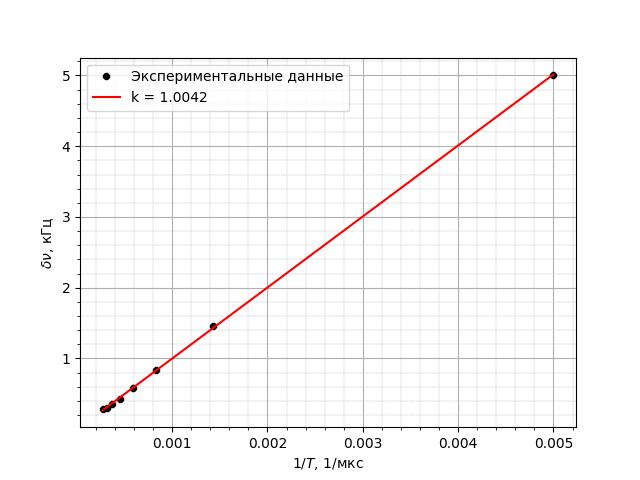
\includegraphics[width=20cm]{image2.jpg}
        \end{center}
        \caption{График зависимости $B(I)$}
        \label{plot1}
    \end{figure}

    По наклонам полученных прямых рассчитаем величину $\chi$ по формуле

    \[ \Delta P = \alpha \cdot B^2 \text{, где } \alpha = \frac{\chi s}{2\mu_0} \text{, где } \mu_0 = 4\pi \cdot 10^{-7} \text{ } \frac{\text{Гн}}{\text{м}} \]
    \[ \Longrightarrow \chi = \frac{2\alpha\mu_0}{s}, \text{ } \sigma_{\chi} = \chi\sqrt{\left(\frac{\sigma_{\alpha}}{\alpha}\right)^2 + \left(\frac{\sigma_{s}}{s}\right)^2} \]

    Результаты вычислений занесём в таблицу \ref{tab3}.

    Результаты, полученные нами, соизмеримы с табличными значениями. Так же совпадает знак, по которому можем определить, к какому типу магнетиков относится образец. Если магнитная восприимчивость со знаком \textbf{минус}, то перед нами \textbf{диамагнетики}, которые в нашем опыте выталкивались полем. Если же, наоборот, магнитная восприимчивость со знаком \textbf{плюс}, то перед нами \textbf{парамагнетики} - втягивались полем.

    \begin{table}[h]
	\centering
	\begin{tabular}{|c|c|c|c|c|c|c|c|}
		\hline
            \multicolumn{8}{|c|}{$W, \text{ } d = (1.0 \pm 0.01) \text{ см}$} \\ \hline
            \hline
		&$\alpha, \text{ }\cdot10^{-4}\frac{\text{Н}}{\text{Тл}^2}$ & $\sigma_{\alpha}, \text{ }\cdot10^{-4}\frac{\text{Н}}{\text{Тл}^2}$ & $\varepsilon_{\alpha}, \%$ & $\chi, \cdot10^{-6}$ & $\sigma_{\chi}, \cdot10^{-6}$ & $\varepsilon_{\chi}, \%$ & $\chi_{tab}, \cdot10^{-6}$ \\ \hline
        - & 23.867 & 0.156 & 0.7 & 76.375 & 1.607 & 2.1 & 68 \\ \hline
        -. & 24.159 & 0.364 & 1.5 & 77.31 & 1.935 & 2.5 & 68 \\ \hline
	\end{tabular}
        \begin{tabular}{|c|c|c|c|c|c|c|c|}
		\hline
            \multicolumn{8}{|c|}{$Cu, \text{ } d = (1.0 \pm 0.01) \text{ см}$} \\ \hline
            \hline
		&$\alpha, \text{ }\cdot10^{-4}\frac{\text{Н}}{\text{Тл}^2}$ & $\sigma_{\alpha}, \text{ }\cdot10^{-4}\frac{\text{Н}}{\text{Тл}^2}$ & $\varepsilon_{\alpha}, \%$ & $\chi, \cdot10^{-6}$ & $\sigma_{\chi}, \cdot10^{-6}$ & $\varepsilon_{\chi}, \%$ & $\chi_{tab}, \cdot10^{-6}$ \\ \hline
        - & -2.964 & 0.026 & -0.9 & -9.485 & -0.208 & 2.2 & -9.8 \\ \hline
        -. & -2.904 & 0.035 & -1.2 & -9.292 & -0.216 & 2.3 & -9.8 \\ \hline
        \end{tabular}
        \begin{tabular}{|c|c|c|c|c|c|c|c|}
		\hline
            \multicolumn{8}{|c|}{$C1, \text{ } d = (0.86 \pm 0.01) \text{ см}$} \\ \hline
            \hline
		&$\alpha, \text{ }\cdot10^{-4}\frac{\text{Н}}{\text{Тл}^2}$ & $\sigma_{\alpha}, \text{ }\cdot10^{-4}\frac{\text{Н}}{\text{Тл}^2}$ & $\varepsilon_{\alpha}, \%$ & $\chi, \cdot10^{-6}$ & $\sigma_{\chi}, \cdot10^{-6}$ & $\varepsilon_{\chi}, \%$ & $\chi_{tab}, \cdot10^{-6}$ \\ \hline
        - & -32.25 & 0.187 & -0.6 & -139.533 & -3.344 & 2.4 & - \\ \hline
        -. & -32.691 & 0.322 & -1.0 & -141.445 & -3.572 & 2.5 & - \\ \hline
	\end{tabular}
        \begin{tabular}{|c|c|c|c|c|c|c|c|}
		\hline
            \multicolumn{8}{|c|}{$Al, \text{ } d = (1.0 \pm 0.01) \text{ см}$} \\ \hline
            \hline
		&$\alpha, \text{ }\cdot10^{-4}\frac{\text{Н}}{\text{Тл}^2}$ & $\sigma_{\alpha}, \text{ }\cdot10^{-4}\frac{\text{Н}}{\text{Тл}^2}$ & $\varepsilon_{\alpha}, \%$ & $\chi, \cdot10^{-6}$ & $\sigma_{\chi}, \cdot10^{-6}$ & $\varepsilon_{\chi}, \%$ & $\chi_{tab}, \cdot10^{-6}$ \\ \hline
        - & 6.363 & 0.055 & 0.9 & 20.363 & 0.444 & 2.2 & 23 \\ \hline
        -. & 6.307 & 0.121 & 1.9 & 20.183 & 0.559 & 2.8 & 23 \\ \hline
        \end{tabular}
	\caption{Результаты вычислений}
	\label{tab3}
    \end{table}
    
\end{enumerate}

\section{Подведение результатов и выводы}

В этой работе мы измерили магнитную восприимчивость образцов, оценили погрешность измерений. Мы получили значения, близкие к табличным. Исходя из результатов, можно сказать, что \textbf{W} и \textbf{Al} -- \textbf{парамагнетики}, а \textbf{Cu} и \textbf{C1} -- \textbf{диамагнетики}.

\begin{table}[h]
\centering
\begin{tabular}{|c|c|c|c|c|c|c|c|}
    \hline
    & $W$ & $Cu$ & $C1$ & $Al$ \\ \hline
    $\chi$ & $(76.4 \pm 1.6) \cdot 10^{-6}$ & $(-9.5 \pm 0.2) \cdot 10^{-6}$ & $(-139.5 \pm -3.3) \cdot 10^{-6}$ & $(20.4 \pm 0.4) \cdot 10^{-6}$ \\ \hline
    $\chi_{tab}$ & $68 \cdot 10^{-6}$ & $-9.8 \cdot 10^{-6}$ & - & $23 \cdot 10^{-6}$ \\ \hline
\end{tabular}

\caption{Итоговая таблица}
\label{tab3}
\end{table}

\newpage

\begin{table}[h]
	\centering
	\begin{tabular}{|c|c|c|}
		\hline
            \multicolumn{3}{|c|}{$W, \text{ } d = (1.0 \pm 0.01) \text{ см}$} \\ \hline
            \hline
		$ I, \text{ А}$ & $ B, \text{ Тл}$ & $\Delta P, \cdot10^{-6}\text{ Н}$ \\ \hline
		0.2 & 0.208 & 98.0 \\ \hline
            0.3 & 0.306 & 225.4 \\ \hline
            0.4 & 0.403 & 401.8 \\ \hline
            0.5 & 0.5 & 617.4 \\ \hline
            0.6 & 0.611 & 911.4 \\ \hline
            0.7 & 0.701 & 1166.2 \\ \hline
            0.8 & 0.785 & 1479.8 \\ \hline
            0.9 & 0.875 & 1793.4 \\ \hline
            1.0 & 0.951 & 2136.4 \\ \hline
            1.1 & 1.014 & 2410.8 \\ \hline
            1.0 & 0.951 & 2195.2 \\ \hline
            0.9 & 0.875 & 1901.2 \\ \hline
            0.8 & 0.785 & 1558.2 \\ \hline
            0.7 & 0.701 & 1225.0 \\ \hline
            0.6 & 0.611 & 940.8 \\ \hline
            0.5 & 0.5 & 646.8 \\ \hline
            0.4 & 0.403 & 431.2 \\ \hline
            0.3 & 0.306 & 254.8 \\ \hline
            0.2 & 0.208 & 117.6 \\ \hline
	\end{tabular}
        \begin{tabular}{|c|c|c|}
		\hline
            \multicolumn{3}{|c|}{$Cu, \text{ } d = (1.0 \pm 0.01) \text{ см}$} \\ \hline
            \hline
		$ I, \text{ А}$ & $ B, \text{ Тл}$ & $\Delta P, \cdot10^{-6}\text{ Н}$ \\ \hline
		0.2 & 0.208 & -9.8 \\ \hline
            0.3 & 0.306 & -19.6 \\ \hline
            0.4 & 0.403 & -39.2 \\ \hline
            0.5 & 0.5 & -68.6 \\ \hline
            0.6 & 0.611 & -98.0 \\ \hline
            0.7 & 0.701 & -137.2 \\ \hline
            0.8 & 0.785 & -176.4 \\ \hline
            0.9 & 0.875 & -215.6 \\ \hline
            1.0 & 0.951 & -254.8 \\ \hline
            1.1 & 1.014 & -294.0 \\ \hline
            1.0 & 0.951 & -264.6 \\ \hline
            0.9 & 0.875 & -225.4 \\ \hline
            0.8 & 0.785 & -186.2 \\ \hline
            0.7 & 0.701 & -147.0 \\ \hline
            0.6 & 0.611 & -117.6 \\ \hline
            0.5 & 0.5 & -78.4 \\ \hline
            0.4 & 0.403 & -49.0 \\ \hline
            0.3 & 0.306 & -29.4 \\ \hline
            0.2 & 0.208 & -19.6 \\ \hline
	\end{tabular}
    
        \begin{tabular}{|c|c|c|}
		\hline
            \multicolumn{3}{|c|}{$C1, \text{ } d = (0.86 \pm 0.01) \text{ см}$} \\ \hline
            \hline
		$ I, \text{ А}$ & $ B, \text{ Тл}$ & $\Delta P, \cdot10^{-6}\text{ Н}$ \\ \hline
		0.2 & 0.208 & -137.2 \\ \hline
            0.3 & 0.306 & -284.2 \\ \hline
            0.4 & 0.403 & -519.4 \\ \hline
            0.5 & 0.5 & -793.8 \\ \hline
            0.6 & 0.611 & -1146.6 \\ \hline
            0.7 & 0.701 & -1538.6 \\ \hline
            0.8 & 0.785 & -1960.0 \\ \hline
            0.9 & 0.875 & -2381.4 \\ \hline
            1.0 & 0.951 & -2851.8 \\ \hline
            1.1 & 1.014 & -3263.4 \\ \hline
            1.0 & 0.951 & -2940.0 \\ \hline
            0.9 & 0.875 & -2508.8 \\ \hline
            0.8 & 0.785 & -2048.2 \\ \hline
            0.7 & 0.701 & -1607.2 \\ \hline
            0.6 & 0.611 & -1205.4 \\ \hline
            0.5 & 0.5 & -852.6 \\ \hline
            0.4 & 0.403 & -558.6 \\ \hline
            0.3 & 0.306 & -313.6 \\ \hline
            0.2 & 0.208 & -137.2 \\ \hline
	\end{tabular}
        \begin{tabular}{|c|c|c|}
		\hline
            \multicolumn{3}{|c|}{$Al, \text{ } d = (1.0 \pm 0.01) \text{ см}$} \\ \hline
            \hline
		$ I, \text{ А}$ & $ B, \text{ Тл}$ & $\Delta P, \cdot10^{-6}\text{ Н}$ \\ \hline
		0.2 & 0.208 & 29.4 \\ \hline
            0.3 & 0.306 & 58.8 \\ \hline
            0.4 & 0.403 & 107.8 \\ \hline
            0.5 & 0.5 & 166.6 \\ \hline
            0.6 & 0.611 & 235.2 \\ \hline
            0.7 & 0.701 & 313.6 \\ \hline
            0.8 & 0.785 & 392.0 \\ \hline
            0.9 & 0.875 & 480.2 \\ \hline
            1.0 & 0.951 & 578.2 \\ \hline
            1.1 & 1.014 & 637.0 \\ \hline
            1.0 & 0.951 & 578.2 \\ \hline
            0.9 & 0.875 & 499.8 \\ \hline
            0.8 & 0.785 & 421.4 \\ \hline
            0.7 & 0.701 & 333.2 \\ \hline
            0.6 & 0.611 & 245.0 \\ \hline
            0.5 & 0.5 & 186.2 \\ \hline
            0.4 & 0.403 & 117.6 \\ \hline
            0.3 & 0.306 & 68.6 \\ \hline
            0.2 & 0.208 & 39.2 \\ \hline
	\end{tabular}
        
	\caption{Результаты измерений}
	\label{tab2}
\end{table}

\end{document}
